% =============================================================================
% Electron thruster for LEO station keeping -- short concept paper
% Build: pdflatex main.tex  (twice for refs)
% The long version (full ladder, characterization, CubeSat scaling, comparison
% with flown micropropulsion) is in git history at commit 6af0807; its content
% lives on in README.md, paper/SCALING_LAWS.md and model/README.md. Every number
% is a committed measurement or model output unless labelled an estimate.
% =============================================================================
\documentclass[11pt,twocolumn]{article}
\usepackage[a4paper,margin=1.5cm,columnsep=0.2in]{geometry}
\usepackage{times}
\usepackage{amsmath,amssymb,graphicx,booktabs,xcolor,url}
\usepackage[hidelinks]{hyperref}
\usepackage{caption}
\usepackage{orcidlink}
\captionsetup{font=small,labelfont=bf}
\setlength{\parskip}{2pt}
\setlength{\textfloatsep}{8pt plus 2pt minus 2pt}
\setlength{\dbltextfloatsep}{8pt plus 2pt minus 2pt}
\setlength{\abovecaptionskip}{4pt}
\newcommand{\fesc}{f_{\mathrm{esc}}}
\newcommand{\mytitle}{Propellantless electron thruster for LEO station keeping}

\title{\Large\bfseries \mytitle}
\author{Ricardo Sebasti\'an Casimiro\,\orcidlink{0009-0008-5188-1326}\\
\normalsize contact: stm32f303ret6@gmail.com}
\date{}

\begin{document}

\twocolumn[
\begin{center}
\maketitle
\begin{abstract}
\noindent
Chip-scale spacecraft lose their orbit to drag faster than any other class and carry no propulsion. This paper presents a thruster with no propellant, tank, feed system or neutralizer: a cathode held a few hundred volts below the spacecraft body emits an electron beam through an aperture, the positively charged body collects the same current back from the ionosphere, and the circuit closes with zero net mass flow. Particle-in-cell simulations (WarpX) of a 10\,mm conducting body in a dayside ionospheric plasma measure 3.4--43\,nN of thrust from 12--278\,mW of beam power over 100--350\,V, with 96--99\,\% of the beam escaping and two measured constants describing every run to within 3\,\%. Against a year of real drag on a sun-synchronous orbit, a 3\,g body 30\,mm long that re-enters from 550\,km in 11 months without the thruster holds its altitude with it for 20\,mW of mean beam power near solar maximum and under 1\,mW near minimum; across 500--700\,km the mean demand is 0.7--9\,nN near maximum and 10--22 times lower near minimum. Drag and collection both scale with area, so the concept carries to CubeSats: a 1U needs about 1\,W at 600\,km near solar maximum, an estimate in a collection regime not yet simulated.
\end{abstract}
\end{center}
\vspace{0.4cm}
]

\section{Introduction}

The smallest spacecraft lose their orbit fastest, because drag grows with area and inertia with volume. KickSat-2 released 105 chip-scale ``Sprites'' of 4\,g each in 2019; they stayed in orbit only a few days \cite{kicksat}. The thrust needed to hold such a craft up is nanonewtons, below anything flown: flight micropropulsion (cold gas, pulsed plasma, electrospray, FEEP) spends a stored propellant through tanks, valves and feed lines, and none of it fits a gram-scale spacecraft \cite{nasasoa26}.

This paper presents a thruster made of a cathode, an aperture and a high-voltage supply, with the ionosphere as the return path. An electron beam carries about 200 times less momentum per watt than an ion beam, which rules the idea out at millinewtons; at the nanonewton demand of a chip-scale spacecraft it costs milliwatts.

\section{Concept}

\begin{figure*}[t]\centering
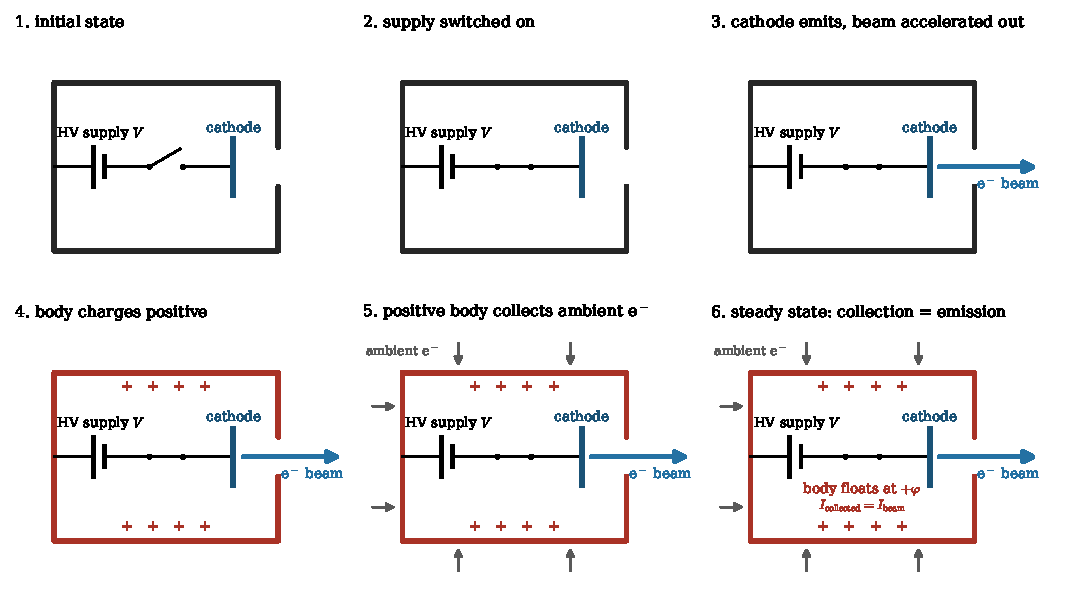
\includegraphics[width=0.88\textwidth]{imgs/concept_steps_mpl.pdf}
\caption{Operating sequence. The supply is switched on, the cathode emits, the escaping beam charges the body positive, and the positive body collects ambient electrons until collection equals emission.}
\label{fig:concept}
\end{figure*}

A cathode held at $-V$ with respect to the spacecraft body emits electrons and accelerates them out through an aperture (Fig.~\ref{fig:concept}). Each escaping electron leaves the body one charge more positive, so the body's conducting skin collects ambient electrons from the plasma, and the supply returns them to the cathode. The body settles at the floating potential $\varphi$ where collection equals emission. The beam is not recaptured: its electrons carry 100--300\,eV, while $\varphi$ is a few to a few tens of volts and the ambient electrons carry 0.1\,eV. The collected electrons arrive from all directions and cancel 0.4--1.4\,\% of the beam thrust at 200--350\,V.

\section{Theory}

The beam is a current $I$ of electrons with kinetic energy KE; its momentum flux is the thrust
\begin{equation}
F = \frac{I\sqrt{2m_e\,\mathrm{KE}}}{e}, \qquad \mathrm{KE} = \kappa\,e\,(V-\varphi),
\label{eq:thrust}
\end{equation}
where the float $\varphi$ is taxed from the supply $V$. The body collects the thermal electron flux enhanced by its potential,
\begin{equation}
I = \beta\,e A n_e\sqrt{\frac{kT_e}{2\pi m_e}}\,\left(1+\frac{e\varphi}{kT_e}\right)^{\alpha},
\label{eq:oml}
\end{equation}
with $\alpha = 1$ for a sphere and $0.5$ for a long cylinder in orbital-motion-limited theory \cite{san93}. Setting $I$ equal to the escaping current gives the float: thin night-side plasma raises it. With $P = VI$, the thrust per watt is $F/P \approx 3.37\sqrt{\kappa/V}$\,\textmu N/W, about 0.2\,\textmu N/W at 200\,V; at fixed thrust, power grows as $\sqrt{V}$, so the lowest voltage that still meets the demand is the cheapest.

\section{Simulated capability}

The device is simulated with WarpX \cite{warpx22,amrex19} in RZ electrostatic mode: a closed 10\,mm can with a cathode disk inside and an aperture in the lid, in a dayside 400\,km plasma ($n_e = 1.63\times10^{12}$\,m$^{-3}$, $kT_e = 114$\,meV, ions at $400\,m_e$), 0.15\,mm cells, 800\,ns runs. The body potential is not prescribed: each step it moves by the net charge that left and landed over the body's self-capacitance. A ladder of nine stages builds from a vacuum electron gun to the full device, checking each piece against theory (thermal collection within 1\,\%); all pass, and every run passes fixed gates on escape, current balance and momentum. Table~\ref{tab:envelope} gives the operating envelope. Two constants describe it: $F = 3.27\,I\sqrt{\mathrm{KE}}$ (97\,\% of Eq.~\ref{eq:thrust}, the rest plume divergence) and $\kappa = 0.81$. Stretching the can to 30\,mm ($L/r = 6$) multiplies its skin by 3.5 at the same frontal area: the float drops fourfold and thrust rises. A 3D run with the geomagnetic field across the beam at flight strength changes the thrust by under 1\,\%.

$\kappa = 0.81$ is a property of the simulation, not the device: the beam is launched 0.3\,mm above the cathode, where the potential is already 19\,\% of $V$ above it, and the measured deficit is 17--18\,\% of $V$ in every run. A real cathode emits at cathode potential ($\kappa \approx 1$), so every thrust and power figure here is conservative by about 11\,\%; a confirmation run is under way.

\begin{table}[t]\centering\small\setlength{\tabcolsep}{4pt}
\caption{Measured operating envelope. $\eta = \mathrm{KE}\,\fesc/eV$. Grid uncertainty: $F \pm 4$\,\%, $\varphi \pm 2$\,\%.}
\label{tab:envelope}
\begin{tabular}{@{}lrrrrrrr@{}}
\toprule
body & $V$ & $I$ & $\varphi$ & $F$ & $P$ & $\fesc$ & $\eta$ \\
& V & mA & V & nN & mW & \% & \\
\midrule
compact & 100 & 0.121 & 5.4  & 3.42  & 12.1 & 96.1 & 0.74 \\
$10\times5.5$\,mm & 200 & 0.342 & 17.0 & 13.65 & 68.4 & 98.4 & 0.73 \\
& 300 & 0.630 & 36.3 & 30.13 & 189  & 99.0 & 0.69 \\
& 350 & 0.793 & 48.3 & 40.48 & 278  & 99.1 & 0.68 \\
\midrule
slender & 200 & 0.342 & 4.4  & 14.22 & 68.4 & 98.4 & 0.79 \\
$10\times30$\,mm & 350 & 0.793 & 14.0 & 43.33 & 278  & 99.1 & 0.77 \\
\bottomrule
\end{tabular}
\end{table}

\section{Station keeping}

\begin{table*}[t]\centering\small
\caption{Station keeping on a sun-synchronous orbit (10:30 ascending node). Each cell is 2024 (near solar maximum) / 2019 (near minimum). Drag is the year-mean thrust demand; lifetime is the free fall with the thruster off, to 120\,km or the 5-year cap; power is the year-mean beam power to hold the altitude. The 1U drag is exact (drag scales with drag area, $\times103$); its power is an estimate scaled the same way. $^\dagger$47\,\% of the points need more than 350\,V: at the edge of the simulated envelope.}
\label{tab:mission}
\begin{tabular}{@{}lrrrrrr@{}}
\toprule
& \multicolumn{3}{c}{3\,g slender can ($10\times30$\,mm)} & \multicolumn{3}{c}{1U CubeSat (1.33\,kg), estimate} \\
\cmidrule(lr){2-4}\cmidrule(lr){5-7}
altitude & drag [nN] & lifetime, off & power [mW] & drag [\textmu N] & lifetime, off & power [W] \\
\midrule
400\,km & 38 / 3.8 & 46\,d / 241\,d & 278$^\dagger$ / 21 & 3.9 / 0.39 & 167\,d / 2.4\,yr & 29$^\dagger$ / 2.2 \\
500\,km & 8.6 / 0.49 & 204\,d / 3.5\,yr & 46 / 2.0 & 0.89 / 0.050 & 2.1\,yr / $>5$\,yr & 4.8 / 0.20 \\
550\,km & 4.3 / 0.21 & 329\,d / 4.5\,yr & 20 / 0.78 & 0.45 / 0.021 & $>5$\,yr / $>5$\,yr & 2.1 / 0.080 \\
600\,km & 2.3 / 0.10 & 2.2\,yr / $>5$\,yr & 9.6 / 0.37 & 0.23 / 0.010 & $>5$\,yr / $>5$\,yr & 0.98 / 0.039 \\
650\,km & 1.2 / 0.057 & $>5$\,yr / $>5$\,yr & 4.8 / 0.21 & 0.12 / 0.006 & $>5$\,yr / $>5$\,yr & 0.49 / 0.022 \\
700\,km & 0.66 / 0.037 & $>5$\,yr / $>5$\,yr & 2.5 / 0.14 & 0.068 / 0.004 & $>5$\,yr / $>5$\,yr & 0.26 / 0.014 \\
\bottomrule
\end{tabular}
\end{table*}

Drag and the plasma along the orbit come from a year-long TudatPy propagation \cite{tudat} with NRLMSISE-00 density \cite{msis} driven by measured solar and geomagnetic indices and IRI-2020 plasma \cite{iri} along the orbit, near solar maximum (2024) and minimum (2019). The test body is the slender can of Table~\ref{tab:envelope}, 3.1\,g, flown with its axis along the velocity, so the thrust axis and the low-drag pose coincide. With the thruster on, drag is cancelled exactly and the drag at each 5-minute point is the thrust demand; the supply voltage follows it at the least beam power, with the float solved from the plasma at that point through Eqs.~\ref{eq:thrust}--\ref{eq:oml}. With the thruster off, the orbit decays freely.

Table~\ref{tab:mission} gives the result. Without the thruster the 3\,g body re-enters from 400\,km in 46 days and from 550\,km in 11 months near solar maximum. With it, 500--700\,km is held all year: the mean demand of 0.7--9\,nN sits inside the measured envelope, for 2.5--46\,mW near maximum and under 2\,mW near minimum. At 400\,km near maximum the 38\,nN mean is below the 43\,nN measured at 350\,V, but the thin night-side plasma pushes half the points past 350\,V; near minimum 400\,km is held for 21\,mW. The ISS and equatorial orbits differ from the sun-synchronous one by about 10\,\%.

The demand is not steady. It swings about $1.7\times$ over each orbit (day and night) and up to $2.5$--$2.8\times$ on storm days (11 May and 7--11 October 2024). Holding altitude is an impulse budget, so the peaks cost a small dip, not the orbit: replayed with thrust capped at the measured 350\,V capability, the orbit never drops more than 10\,m below its target at 500--700\,km.

Drag, current and beam power all scale with the drag area, so the concept does not depend on size. A 1U CubeSat has 103 times the can's drag area and needs 103 times its thrust and, to first order, its power: about 1\,W at 600\,km near solar maximum and tens of milliwatts near minimum. A 1U lives longer in free fall because its mass grows faster than its area: 167 days from 400\,km near solar maximum, against 46 for the can.

\section{Limitations}
\begin{enumerate}\setlength{\itemsep}{1pt}
  \item \textbf{Settling.} Ions are $400\,m_e$ and floats are 800\,ns snapshots; a 3D campaign settled its floats at 6\,\textmu s at about twice the 800\,ns value, with thrust moving by a few percent.
  \item \textbf{Prescribed beam.} Beam current is an input, launched above the cathode ($\kappa$ above); the flight emitter is not chosen.
  \item \textbf{CubeSat regime.} The simulated body is 2.5 Debye lengths across; a 1U is about 25, where Eq.~\ref{eq:oml} is not measured.
  \item \textbf{Attitude and plasma flow.} A held pose is assumed and the plasma is stationary (no ram flow).
\end{enumerate}
All powers are beam power $VI$; converter and cathode overheads belong to the flight design.

\section{Conclusion}
A cathode, a high-voltage supply and the spacecraft's own skin make a thruster that needs no propellant. Simulations measure 3.4--43\,nN from 12--278\,mW, enough to hold a 3\,g chip-scale spacecraft at 500--700\,km for milliwatts where it would otherwise re-enter within a year, and the same physics scales with area to CubeSats at around a watt. The next steps are a settled, cathode-launched confirmation run and a large-body run in the CubeSat regime.

\paragraph{Data.} Simulation inputs, run manifests, gate policies, orbit propagations and the model are in the project repository, archived at \href{https://doi.org/10.5281/zenodo.22115924}{DOI:10.5281/zenodo.22115924}.

\paragraph{Acknowledgements.} This research used the open-source \href{https://blast-warpx.github.io}{particle-in-cell code WarpX}. Primary WarpX contributors are with LBNL, LLNL, CEA-LIDYL, SLAC, DESY, CERN, Helion Energy, TAE Technologies, and Realta Fusion. We acknowledge all WarpX contributors. Orbit propagation used TudatPy.

\begin{thebibliography}{99}\footnotesize\setlength{\itemsep}{0pt}
\bibitem{kicksat} S.~Kacapyr, ``Cracker-sized satellites demonstrate new space tech,'' \emph{Cornell Chronicle}, 3 June 2019.
\bibitem{nasasoa26} NASA, ``State of the Art of Small Spacecraft Technology,'' 2026 ed., Ch.~4.
\bibitem{san93} J.~R.~Sanmart\'in, M.~Mart\'inez-S\'anchez, E.~Ahedo, ``Bare wire anodes for electrodynamic tethers,'' \emph{J. Propulsion and Power} 9(3), 353--360, 1993.
\bibitem{warpx22} J.-L.~Vay et al., ``WarpX: An advanced Particle-In-Cell code,'' version 26.05, Zenodo, DOI:10.5281/zenodo.4571577, \url{https://blast-warpx.github.io}.
\bibitem{amrex19} W.~Zhang et al., ``AMReX: a framework for block-structured adaptive mesh refinement,'' \emph{J. Open Source Software} 4(37), 1370, 2019.
\bibitem{tudat} Tudat Space (TudatPy), TU Delft Astrodynamics Toolbox, \url{https://docs.tudat.space}.
\bibitem{msis} J.~M.~Picone, A.~E.~Hedin, D.~P.~Drob, A.~C.~Aikin, ``NRLMSISE-00 empirical model of the atmosphere: statistical comparisons and scientific issues,'' \emph{J. Geophys. Res.} 107(A12), 1468, 2002.
\bibitem{iri} D.~Bilitza et al., ``The International Reference Ionosphere model: a review and description of an ionospheric benchmark,'' \emph{Rev. Geophys.} 60, e2022RG000792, 2022.
\end{thebibliography}

\end{document}
